\documentclass{beamer}
\usepackage[utf8]{inputenc}
\usepackage{epstopdf}
\usepackage{animate}
\usepackage{pgfpages}
\usepackage{media9}
\usepackage{cases}
\graphicspath{{img/}}
\usepackage{tikz}
\usetikzlibrary{arrows,shapes,trees,patterns,arrows,decorations.pathreplacing}
%\setbeameroption{show notes on second screen}
\usetheme[pageofpages=/,% String used between the current page and the
                         % total page count.
          bullet=circle,% Use circles instead of squares for bullets.
          titleline=true,% Show a line below the frame title.
          alternativetitlepage=true,% Use the fancy title page.
          titlepagelogo=logo_afonso,% Logo for the first page.
          watermark=Minerva_UFRJ_Black_transparency,% Watermark used in every page.
          watermarkheight=90px,% Height of the watermark.
          watermarkheightmult=4,% The watermark image is 4 times bigger
                                % than watermarkheight.
          ]{Torino}
\usepackage[brazil]{babel}

\author{\textbf{Alunos: \newline
		Cayo Valsamis \newline
		Gabriel Pelielo \newline
		Rafael Accácio \newline
		Rodrigo Moysés}}
\title{\textbf{Introdução à Otimização \vspace{0.25cm} \newline 
		       Trabalho Final}}
\institute{Universidade Federal do Rio de Janeiro}
\date{01 de Dezembro, 2015}


\begin{document}
	
	\setbeamertemplate{section in toc}[square]
	
	\AtBeginSection[]{
		\begin{frame}
			\frametitle{Sumário}
			\tableofcontents[currentsection]
		\end{frame}
	}
	
	
	\begin{frame}[t,plain]
		\titlepage
	\end{frame}
	
	\begin{frame}{Sumário}
		\tableofcontents
	\end{frame}
	
\section{Mínimos Quadrados}
\begin{frame}[t]{Mínimos Quadrados}
	\begin{itemize}
	\item Minimizar Quadrado dos Resíduos
	\end{itemize}\pause
	\begin{equation}
min(\sum^n (\mathbf{f}(t_k,\omega_n,\zeta)-\mathbf{y}_k))
\end{equation}\pause
\begin{itemize}
	\item $n$ é o número de amostras.\pause
	\item $k$ é uma amostra.\pause
	\item $\mathbf{f}(t_k,\omega_n,\zeta)$ é a expressão da função de resposta no tempo k.\pause
	\item $t_k$ é o instante de tempo da k-ésima amostra.\pause
	\item $\mathbf{y}_k$ é o valor medido na amostra $k$.\pause
	\item $\omega_n$ e $\zeta$ são os parâmetros do sistema.
	\note<8>{ZETA}
	\end{itemize}
\end{frame}

\begin{frame}[t]{"Dividir e Conquistar"}
\only<1-2>{Iremos dividir em duas partes}
\begin{enumerate}
\item<1-2> Calcular a expressão $\sum_{i=1}^k (\mathbf{f}(t_k,\omega_n,\zeta)-\mathbf{y}_k)$\pause
\item<2> Minimizar a expressão através de algum método.
\end{enumerate}
\only<3>{\vspace{-1cm}Quais métodos?}
\only<4-6>{Métodos Antigos?\\}
\only<5-6>{ \vspace{1cm}\hspace{3cm}Métodos Novos?\\}
\only<6>{ \vspace{1cm}\hspace{6cm}Veremos...}
\end{frame}

\section{Algoritmo Genético}
\begin{frame}[t]{Algoritmo Genético}
	
	O algoritmo genético é inspirado pelo evolucionismo, que se baseia em gerações de indivíduos, em que os mais aptos prevalecem e constroem a geração futura.
	
	\begin{figure}[h]
		\begin{center}
			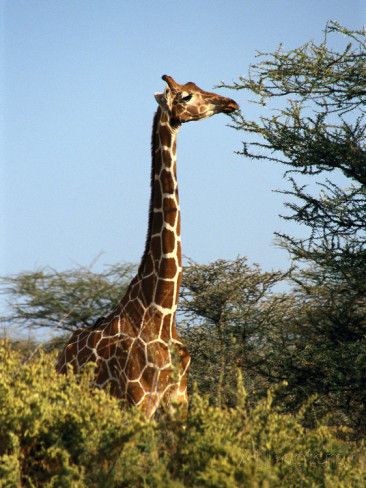
\includegraphics[width=3cm]{./giraffe.jpg}   
		\end{center}
	\end{figure}
	
\end{frame}

\begin{frame}[t]{Algoritmo Genético}
	
	O primeiro passo para a construção do algoritmo genético é a criação de uma \textbf{primeira geração}, feita aleatoriamente, com quantidade de indivíduos e limites definidos.
	
		\begin{center}
			\animategraphics[autoplay,loop,width=5cm]{1}{frame_}{1}{5}
		\end{center}
	
\end{frame}
	
\begin{frame}[t]{Algoritmo Genético}
	O segundo passo é criar a \textbf{população intermediária}. O método escolhido para tal foi o canônico, com aptidão definida como 
	
	\begin{equation*}
		\phi_i = \dfrac{\bar{f}}{f_i}
	\end{equation*}
	
	Sendo
	\begin{itemize}
		\item $ \phi_i $ a aptidão do indivíduo $ i $.
		\item $ f_i $ a função objetivo avaliada no ponto do indivíduo $ i $.
		\item $ \bar{f} $ a média do valor da função para toda a população.
	\end{itemize} 
	
\end{frame}

\begin{frame}[t]{Algoritmo Genético}
	
	O terceiro passo é a recombinação, processo necessário para construir a \textbf{segunda geração}. O tipo de recombinação escolhido foi a média de três pais, para acelerar a convergência.
	
	\begin{figure}[h]
		\begin{center}
		\begin{tikzpicture}[scale = 0.65]
		
		
		\draw  (-5.0,4.0) rectangle (-1.5,-2.5);
		\draw  (0.0,4.0) rectangle (3.5,-2.5);
		\draw  (5.0,4.0) rectangle (8.5,-2.5);
		
		\draw [] (-5,3.2) -- (-1.5,3.2);
		\draw [] (-5,2.4) -- (-1.5,2.4);
		\draw [] (-5,1.6) -- (-1.5,1.6);
		\draw [] (-5,0.8) -- (-1.5,0.8);
		\draw [] (-5,0) -- (-1.5,0);
		
		\node at (-3.2,3.5) {Pai 1};
		\node at (-3.2,2.7) {Pai 2};
		\node at (-3.2,1.9) {Pai 3};
		\node at (-3.2,1.1) {Pai 4};
		\node at (-3.2,0.3) {...};
		
		\draw [dashed, -stealth] (-1.5,3.5) -- (0,3.5);
		\draw [dashed, -stealth] (-1.5,1.9) -- (0,2.7);
		\draw [dashed, -stealth] (-1.5,1.9) -- (0,1.9);
		\draw [dashed, -stealth] (-1.5,1.1) -- (0,1.1);
		
		\draw [] (0,3.2) -- (3.5,3.2);
		\draw [] (0,2.4) -- (3.5,2.4);
		\draw [] (0,1.6) -- (3.5,1.6);
		\draw [] (0,0.8) -- (3.5,0.8);
		\draw [] (0,0) -- (3.5,0);
		
		\node at (1.8,3.5) {Pai 1};
		\node at (1.8,2.7) {Pai 3};
		\node at (1.8,1.9) {Pai 3};
		\node at (1.8,1.1) {Pai 4};
		\node at (1.8,0.3) {...};
		
		\draw [] (5,3.2) -- (8.5,3.2);
		\draw [] (5,2.4) -- (8.5,2.4);
		\draw [] (5,1.6) -- (8.5,1.6);
		\draw [] (5,0.8) -- (8.5,0.8);
		\draw [] (5,0) -- (8.5,0);
		
		\node at (6.8,3.5) {Filho 1};
		\node at (6.8,2.7) {Filho 2};
		\node at (6.8,1.9) {Filho 3};
		\node at (6.8,1.1) {Filho 4};
		\node at (6.8,0.3) {...};
		
		
		\node at (-0.8,4.6) {Seleção};
		\node at (4.2,4.6) {Recombinação};
		
		
		\node at (-3.2,-3) {Primeira geração};
		\node at (1.8,-3) {Geração intermediária};
		\node at (6.8,-3) {Segunda geração};
		
		\draw [decorate,decoration={brace,amplitude=10pt},xshift=0.4pt,yshift=-0.4pt](3.5,3.9) -- (3.5,1.7);
		\draw [decorate,decoration={brace,amplitude=10pt},xshift=0.4pt,yshift=-0.4pt](3.5,1.5) -- (3.5,-0.7);
		\draw [dashed, -stealth] (3.9,2.8) -- (5.0,3.5);
		\draw [dashed, -stealth] (3.9,0.4) -- (5.0,2.7);
		
		
		\end{tikzpicture}
			\label{fig:genetico_tikz}		
		\end{center}
	\end{figure}
	
	
	
\end{frame}

\begin{frame}
	
	\begin{figure}[h]
		\begin{center}
			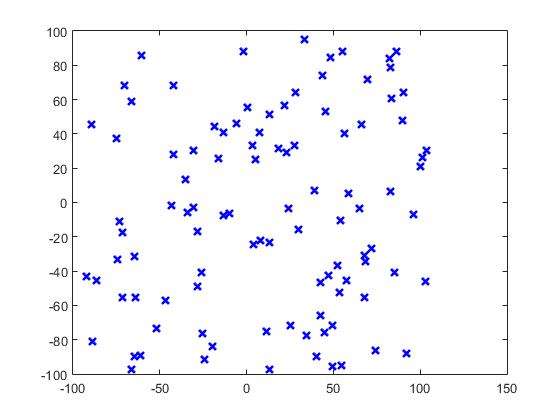
\includegraphics[width=8cm]{./g1.png}   
			\caption{Exemplo de primeira iteração}
			\label{fig:g1}
		\end{center}
	\end{figure}
	
	
\end{frame}

\begin{frame}
	
	\begin{figure}[h]
		\begin{center}
			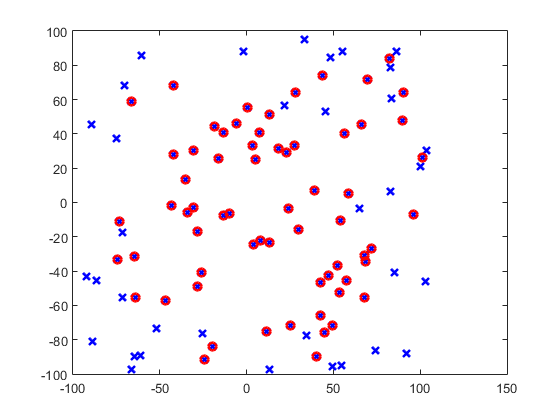
\includegraphics[width=8cm]{./g1_inter.png}   
			\caption{Exemplo de primeira iteração}
			\label{fig:g1_inter}
		\end{center}
	\end{figure}
	
	
\end{frame}

\begin{frame}
	
	\begin{figure}[h]
		\begin{center}
			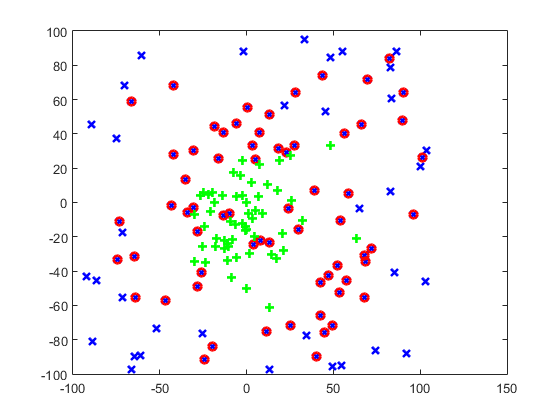
\includegraphics[width=8cm]{./g2.png}   
			\caption{Exemplo de primeira iteração}
			\label{fig:g2}
		\end{center}
	\end{figure}
	
	
\end{frame}
	
	



\section{Simplex}
\begin{frame}[t]{Simplex}
\begin{itemize}
\item Método de minimização multidimensional 
sem restrições
\item John A. Nelder e Roger Mead, 1965 ``The Computer Journal''.
\item Utiliza um Simplex para minimizar uma função de $n$ variáveis. 
\end{itemize}

\note{Também chamado de método Nelder-Mead}
\end{frame}

\begin{frame}[t]{Simplex}
\begin{itemize}
\pause
\item O que é um Simplex?\pause
\end{itemize}
\begin{figure}[h]
	\begin{center}	
		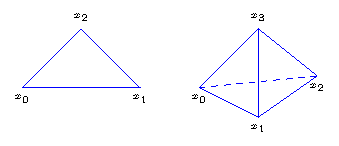
\includegraphics[width=10cm]{simplex/simplex.pdf}
		\caption{Exemplos de Simplex para $\mathbb{R}^2$ e $\mathbb{R}^3$.}
		\label{fig:simplex}
	\end{center}
\end{figure}
\note<1>{Mas a pergunta que não quer calar? O que é um simplex?}
\note<2>{Um Simplex é o menor politopo possível para um espaço de n variáveis. Como exemplo, vemos a figura \ref{fig:simplex}. Para $\mathbb{R}^2$ o menor politopo é um Triângulo, e para $\mathbb{R}^3$ é um Tetraedro.}
\note<3>{Exemplos de simplex}
\end{frame}

\begin{frame}[t]{Simplex}
\begin{itemize}
\item Método Generalista\pause
\item Não Precisa de cálculos complexos\pause
\item Considerado método de ordem $0$
\end{itemize}
\note<1,2>{Este é um método bem generalista que serve para diversos problemas pela sua facilidade, e por não necessitar de Gradientes e Hessianas, como veremos a seguir, é considerado um método de ordem 0.}
\note<3>{Então para facilitar a visualização, representação e entendimento, será explicado o método para $\mathbb{R}^2$}
\end{frame}

\begin{frame}[t]{Divisão do Método}
\pause
\begin{enumerate}
\item Ordenação \pause
\item Busca do Centróide\pause 
\item Reflexão \pause
\item Expansão\pause
\item Contração\pause
\item Encolhimento
\end{enumerate}
\note<7>{Serão explicados nos próximos slides}
\end{frame}

\begin{frame}[t]{Ordenação}
\begin{equation}
x_l=min(f(x_i))
\end{equation}
\begin{equation}
x_h=max(f(x_i)), x_i\neq x_l
\end{equation}
\begin{center}
		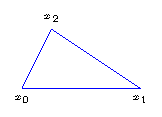
\includegraphics[width=4cm]{simplex/simplex3}
		\includegraphics<2>[width=4cm]{simplex/simplex2}
		
		
		\only<1>{{\usebeamercolor[fg]{caption name}Figura:} Pontos antes da ordenação}
		\only<2>{{\usebeamercolor[fg]{caption name}Figura:} Pontos após ordenação}
\end{center}
\note{\begin{itemize}
\item $x_h$ high
\item $x_l$ low
\item outro $x_s$ arbitrariamente
\end{itemize}}
\end{frame}

\begin{frame}[t]{Busca do Centróide}
\begin{equation}
c=\dfrac{x_l+x_s}{2}
\end{equation}
\begin{center}
		\includegraphics<1>[width=4cm]{simplex/simplex2}
		\includegraphics<2>[width=4cm]{simplex/centroide}
\end{center}
\note{encontra-se o centróide entre todos os pontos excluindo o $x_h$}
\end{frame}

\begin{frame}[t]{Reflexão}
\begin{equation}
x_r=c+\alpha(c-x_h)
\end{equation}
\begin{itemize}
\item $\alpha$=1
\end{itemize}
	
\begin{center}
		\includegraphics<1>[width=4cm]{simplex/centroide}
		\includegraphics<2>[width=4cm]{simplex/reflexao.pdf}
				
		\only<2>{{\usebeamercolor[fg]{caption name}Figura:} Reflexão}
\end{center}	
\end{frame}

\begin{frame}[t]{Reflexão}
\begin{itemize}
\item Se $f(x_l)<f(x_r)<f(x_s)$, $x_h$:=$x_c$\pause
\item Caso contrário, realizar alguma das próximas transformações 
\end{itemize}
\note<1>{Coeficiente de reflexão}
\end{frame}

\begin{frame}{Expansão}
\begin{itemize}
\item Se $f(x_r)<f(x_l)$
\end{itemize}
\begin{equation}
x_e=c+\gamma(x_r-c)
\end{equation}
\begin{itemize}
\item $\gamma$=2
\end{itemize}
\begin{figure}[H]
	\begin{center}	
		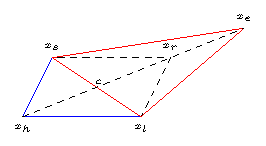
\includegraphics[width=6cm]{simplex/expansao.pdf}
		\caption{Expansão.}
		\label{fig:expansao}
	\end{center}
\end{figure}
\note{Coeficiente de expansão}
\end{frame}

\begin{frame}{Expansão}
\begin{itemize}
\item Se $f(x_r)<f(x_e)$, $x_h$:=$x_r$
\item Se $f(x_e)<f(x_r)$, $x_h$:=$x_e$
\end{itemize}
\note{pega o menor entre eles}
\end{frame}

\begin{frame}[t]{Contração}
\begin{itemize}
\item Se $f(x_r)\geq f(x_l)$
\end{itemize}
\begin{subnumcases}{x_c=}
   c+\beta(x_r-c) & Se $f(x_s)\leq f(x_r)<f(x_h)$ \label{positive}
   \\
   c+\beta(x_h-c) & Se $f(x_r)>f(x_h)$ \label{negative}
\end{subnumcases}
\begin{itemize}
\item $\beta$=$\frac{1}{2}$
\end{itemize}
\begin{figure}[h]
	\begin{center}	
		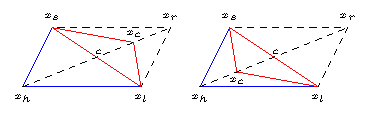
\includegraphics[width=8cm]{simplex/contracao.pdf}
		\caption{Representação das Contrações.}
		\label{fig:contracao}
	\end{center}
\end{figure}
\note<1>{Coeficiente de contração}
\end{frame}

\begin{frame}[t]{Contração}
\[
\text{Contração para fora}
  \begin{cases} 
    \text{Substituir $x_h$ por $x_c$} & \text{Se } f(x_c)\leq f(x_r) \\
   \text{Realizar encolhimento}       & \text{Se } f(x_c)>f(x_r)
  \end{cases}\]
  \[
  \text{Contração para dentro}
  \begin{cases} 
   \text{Substituir $x_h$ por $x_c$} & \text{Se } f(x_c)<f(x_h) \\
   \text{Realizar encolhimento}       & \text{Se } f(x_c)\geq f(x_h)
  \end{cases}
\]
\end{frame}


\begin{frame}[t]{Encolhimento}
\begin{subequations}
\begin{align}
x_s:=x_s+\delta (x_s-x_l)\\
x_h:=x_h+\delta (x_h-x_l)
\end{align}
\end{subequations}
\begin{itemize}
\item $\delta$=$\frac{1}{2}$
\end{itemize}
\begin{figure}[h]
	\begin{center}	
		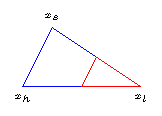
\includegraphics[width=4cm]{simplex/encolher.pdf}
		\caption{Encolhimento.}
		\label{fig:encolher}
	\end{center}
\end{figure}
\note{O encolhimento é muito raro de acontecer e é usado para quando todas as outras transformações anteriores resultam em pontos cujo valor correspondente na função é pior que os anteriores. O que só acontece em casos específicos. Exemplo de caso pode ser visto um extrato da publicação original de 1965
}
\end{frame}

\begin{frame}[t]{Encolhimento}
\begin{quote}
``A failed contraction is much rarer, but can occur when a valley is curved and one point of the simplex is much farther from the valley bottom than the others; contraction may then cause the reflected point to move away from the valley bottom instead of towards it. Further contractions are then useless. The action proposed contracts the simplex towards the lowest point, and will eventually bring all points into the valley.''
\end{quote}
\note{blablablabla....}
\end{frame}

\begin{frame}[t]{Critérios de Parada}
\begin{enumerate}\pause
\item Iterações\pause
\item Raio da circunferência circunscrita
\item<4-5> Desvio Padrão dos $f(x)$
\end{enumerate}
\begin{center}
		\includegraphics<3>[width=5cm]{simplex/parada.pdf}
		\includegraphics<4-5>[width=8cm]{simplex/desviopadrao.pdf}
				
		\only<3>{{\usebeamercolor[fg]{caption name}Figura:} Circunferência circunscrita ao simplex.}
		\only<4>{{\usebeamercolor[fg]{caption name}Figura:} Desvio padrão}
		\only<5>{{\usebeamercolor[fg]{caption name}} Onde $\sigma$=$\sqrt{\frac{\sum_i^n(y_i-\overline{y})^2}{n}}$}
\end{center}
\note<1>{Foram utilizados 3 critérios de parada nesse método}
\note<4>{Cálculo do desvio utilizando três dados por vez. Cada vértice do triângulo a partir da fórmula a seguir}
\note<5>{Quando o desvio chega a zero significa que a superfície se comporta como um plano que não possui mínimo.}
\end{frame}


\section{Conclusão}
bla bla bla

\end{document}


